%! Author = zhiweizhang
%! Date = 10.06.25

\chapter{Model Deployment and \ac{API} Service}\label{chapter:model-deployment-and-api-service}

To facilitate real-world application and integration of the trained classification models, an \ac{API} service was
developed to serve the best-performing models from both the binary and multi-class classification tasks. The service
was designed with a strong emphasis on modularity, portability, and usability.

Although the \ac{API} was not deployed to an online hosting platform due to infrastructure constraints, it was fully
implemented, containerized using Docker, and published to Docker Hub. This approach ensures reproducibility and
allows collaborators (e.g., from the social sciences) or third-party researchers to easily run the service in local
or cloud-based environments supporting Docker runtime.

\section{System Architecture}

\begin{figure}[ht]
    \centering
    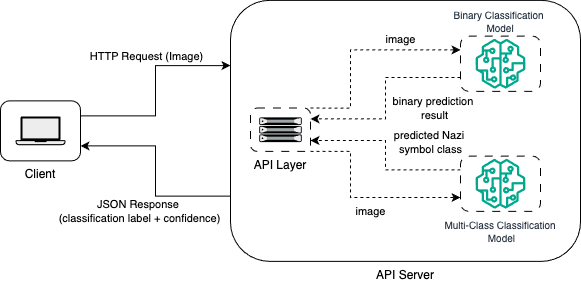
\includegraphics[width=0.7\textwidth]{figures/system_architecture}
    \caption{System architecture of the implemented classification \ac{API} service.}
    \label{fig:system-architecture}
\end{figure}

~\autoref{fig:system-architecture} illustrates the system architecture of the classification \ac{API} service. Users
submit an image file via an HTTP request, which is routed to one of three model pipelines depending on the specified
task: binary classification, multi-class classification, or a two-stage hierarchical classification pipeline.

In the two-stage pipeline, the image is first passed to a binary classifier to determine whether it contains Nazi
symbolism. If no such content is detected, the \ac{API} returns a negative classification. If Nazi-related content
is identified, the image is subsequently forwarded to the multi-class classifier, which predicts the specific type(
s) of Nazi symbol(s), such as swastikas, \ac{SS} bolts, or eagles.

This cascaded design reduces computational overhead for irrelevant inputs and mirrors real-world content moderation
workflows, where fine-grained analysis is only triggered upon initial positive screening.

The backend is implemented using \texttt{FastAPI}. All models are preloaded into memory at service startup, ensuring
low-latency inference. The architecture is stateless and fully containerized, enabling straightforward horizontal
scaling in distributed environments.

\section{Model Integration and Routing Logic}

The \ac{API} exposes distinct endpoints for binary classification, multi-class classification, and the combined
2-layer pipeline. Instead of selecting the model dynamically based on request parameters, each endpoint corresponds
to a specific inference path.

This design simplifies both the server-side routing and the client interface, enabling users to directly interact
with the appropriate endpoint. Each endpoint internally handles preprocessing, model inference, and result formatting.

At service startup, all models are preloaded into memory. \ac{DL} models implemented with PyTorch are
serialized using \texttt{TorchScript}~\footnote{\url{https://pytorch.org/docs/stable/jit.html}} or the standard
PyTorch save format~\footnote{\url{https://pytorch.org/tutorials/beginner/saving_loading_models.html}}.
Classical \ac{ML} models (e.g., logistic regression or \ac{SVC} trained on OpenCLIP embeddings) are serialized using
\texttt{joblib}~\footnote{\url{https://joblib.readthedocs.io/en/latest/}}. This preloading strategy reduces runtime
latency and avoids repeated I/O overhead.

The modular architecture allows easy extension. New models or task-specific pipelines can be integrated by
registering additional routes in the \ac{API} codebase, without disrupting existing functionality.

~\autoref{fig:api-model-routing} summarizes the endpoint-to-model routing logic.

%! Author = zhiweizhang
%! Date = 11.06.25

% Preamble
\begin{figure}[ht]
\centering
\resizebox{\textwidth}{!}{
\begin{tikzpicture}[
    node distance=1.5cm and 2cm,
    every node/.style={font=\small},
    process/.style={rectangle, draw=blue!50, fill=blue!10, thick, minimum width=3.5cm, minimum height=0.9cm},
    endpoint/.style={rectangle, draw=black!80, fill=gray!10, thick, minimum width=4cm, minimum height=0.9cm},
    decision/.style={diamond, aspect=2, draw=red!60, fill=red!10, thick, minimum height=1.2cm},
    response/.style={rectangle, draw=green!50!black, fill=green!10, thick, minimum width=3.5cm, minimum height=0.9cm},
    arrow/.style={->, thick}
]

% API Endpoints
\node[endpoint] (binary) {POST /predict-binary};
\node[endpoint, below=of binary] (multi) {POST /predict-multiclass};
\node[endpoint, below=of multi] (twolayer) {POST /predict};

\node[process, right=of multi] (prep) {Image Preprocessing};

% Two-layer path
\node[decision, right=of prep] (decision) {Contains Nazi Symbol?};
\node[process, right=of decision] (negresponse) {Return: No Symbol};

% Binary path
\node[process, above=2cm of decision] (binarymodel) {Binary Classifier};
\node[response, right=of binarymodel] (binaryresp) {Binary Prediction Response};

% Multi-class path
\node[process, below=2cm of decision] (multimodel) {Multi-Class Classifier};
\node[response, right=of multimodel] (multiresp) {Multi-Class Prediction Response};

\node[response, below right=of multimodel] (finalresp) {Hierarchical Prediction Response};
% Arrows
\draw[red, arrow] (binary.east) -| (prep.150);
\draw[red, arrow] (prep.north) |- (binarymodel.west);
\draw[red, arrow] (binarymodel) -- (binaryresp);

\draw[blue, arrow] (multi) -- (prep);
\draw[blue, arrow] (prep.south) |- (multimodel.west);
\draw[blue, arrow] (multimodel) -- (multiresp);

\draw[arrow] (twolayer.east) -| (prep.-150);
\draw[arrow] (prep) -- (binarymodel);
\draw[arrow] (binarymodel) -- (decision);
\draw[arrow] (decision) -- node[above right] {No} (negresponse);
\draw[arrow] (decision) -- node[below right] {Yes} (multimodel);
\draw[arrow] (multimodel.south) |- (finalresp.west);

\end{tikzpicture}
}
\caption{\ac{API} endpoints mapped to model pipelines, including the 2-layer classification logic.}
\label{fig:api-model-routing}

\end{figure}

\section{Continuous Integration and Deployment}

The service is integrated with a GitHub Actions-based \ac{CI/CD} pipeline, shown in ~\autoref{fig:github-pipeline},
which automates:

\begin{itemize}
    \item Code quality checks and unit testing
    \item Docker image builds and tagging
    \item Generation and deployment of Sphinx-based documentation
    \item Publication of Docker images to Docker Hub
\end{itemize}

Although the \ac{API} is not deployed to a public endpoint, the pipeline ensures that each commit to the main branch
undergoes validation and build procedures, promoting maintainability. Users can reliably pull the latest version
from Docker Hub and execute the service locally or in private cloud environments with minimal setup.

\begin{figure}[ht]
    \centering
    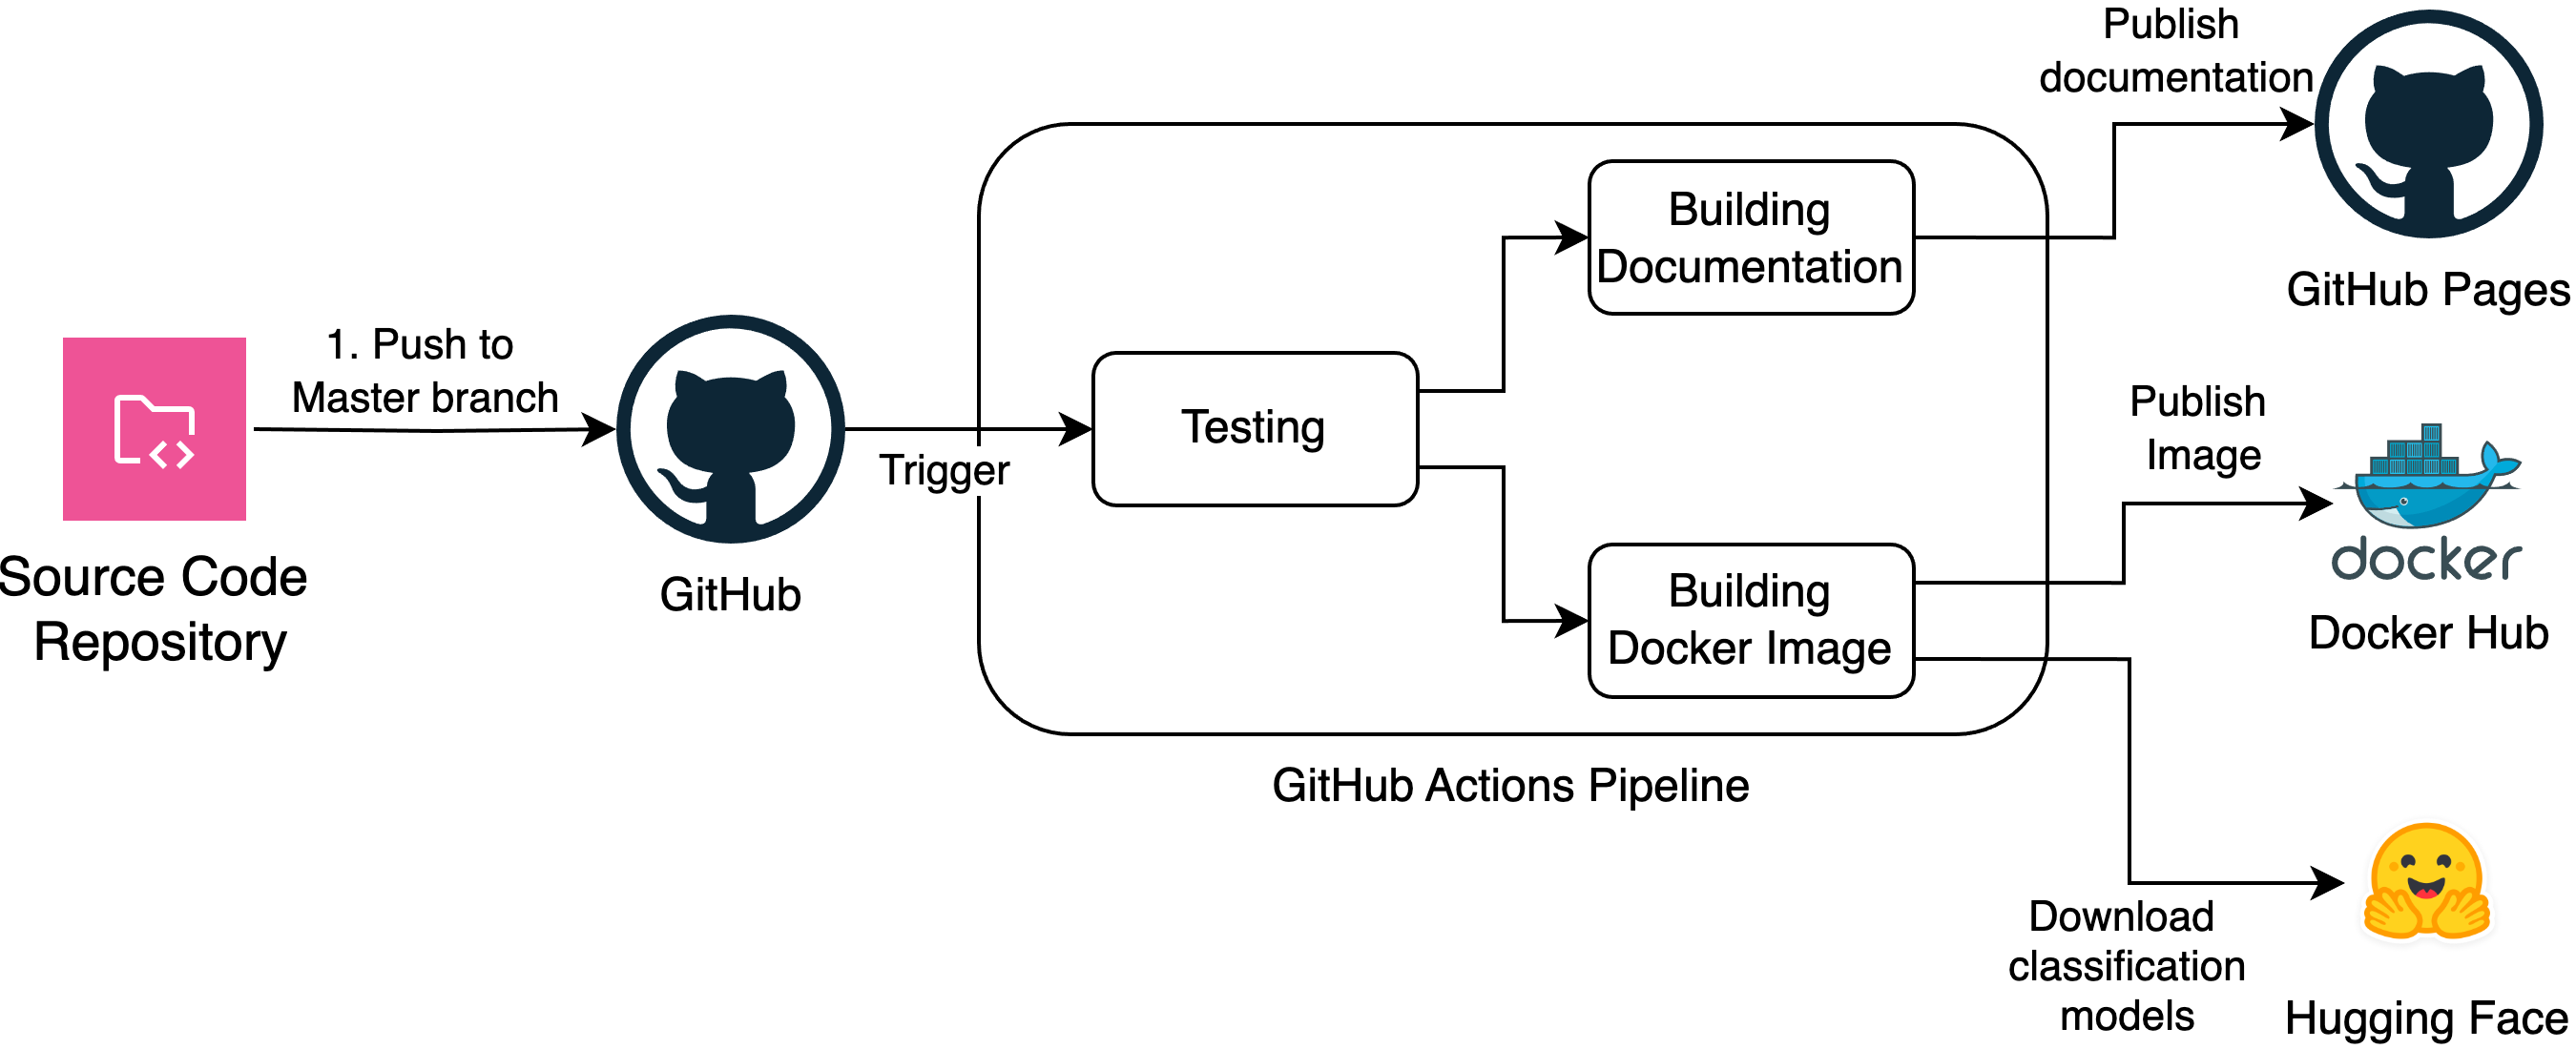
\includegraphics[width=0.7\textwidth]{figures/github_pipeline}
    \caption{GitHub Actions \ac{CI/CD} pipeline for Dockerized \ac{API} service.}
    \label{fig:github-pipeline}
\end{figure}


\section{\ac{API} Endpoints}

\autoref{tab:api-endpoints} summarizes the available endpoints and their functionality.

The 2-layer endpoint encapsulates the binary–multi-class cascade, simplifying client-side logic and supporting
integration into broader moderation or research pipelines.

%! Author = zhiweizhang
%! Date = 10.06.25

% Preamble
\begin{table}[ht]
  \centering
  \resizebox{\textwidth}{!}{
  \begin{tabular}{llp{8cm}}
    \toprule
    \textbf{Method} & \textbf{Endpoint} & \textbf{Description} \\
    \midrule
    \texttt{POST}   & \texttt{/predict} & Runs the 2-layer pipeline: binary classification followed by multi-class prediction if Nazi content is detected. Threshold for symbol inclusion is 0.1. \\
    \texttt{POST}   & \texttt{/predict-binary} & Performs binary classification with associated confidence scores. \\
    \texttt{POST}   & \texttt{/predict-multiclass} & Performs multi-label classification of Nazi symbol types. Returns predictions above confidence threshold 0.1. \\
    \texttt{GET}    & \texttt{/health} & Health check endpoint. \\
    \texttt{GET}    & \texttt{/version} & Returns model and \ac{API} version metadata. \\
    \texttt{GET}    & \texttt{/docs} & Serves OpenAPI documentation via Swagger UI. \\
    \bottomrule
  \end{tabular}
  }
  \caption{Summary of available \ac{API} endpoints.}
  \label{tab:api-endpoints}
\end{table}

All classification endpoints accept images as multipart form data and return structured \ac{JSON} responses. These
responses include predicted classes, confidence scores, and model metadata. The interactive Swagger UI at
\texttt{/docs} facilitates testing and exploration.

\subsection{Example JSON Response}

~\autoref{fig:binary-json-response} shows a sample \ac{JSON} response for the binary classification endpoint.
~\autoref{fig:multi-class-json-response} illustrates a multi-class classification response, while
~\autoref{fig:two-layer-json-response} demonstrates the 2-layer classification response format.

\input{figures/api_responses}

\subsection{Thresholding vs. Top-$k$ in Multi-label Classification}

In the multi-class classification task, images may contain more than one Nazi symbol, constituting a multi-label
problem. Instead of using a top-$k$ strategy, which returns the $k$ most confident classes regardless of absolute
probability, a fixed confidence threshold of 0.1 was used to filter results.

This design offers two key advantages:

\begin{enumerate}
    \item \textbf{Adaptability to Varying Label Counts}: The number of relevant symbols varies across images. A
    threshold-based method allows the model to return only those classes exceeding the confidence threshold, thereby
    adapting to the input's true label count.

    \item \textbf{Reduction of False Positives}: Low-probability predictions are filtered out, reducing the
    likelihood of returning irrelevant or incorrect classifications. This is particularly important in sensitive
    domains such as Nazi symbolism detection, where misclassification could have serious social and legal implications.
\end{enumerate}

This approach provides more nuanced, context-aware predictions and aligns with the goal of responsible content
moderation.

\section{Extensibility and Future Deployment}

The \ac{API} service is architected for extensibility. Future capabilities—such as object detection for symbol
localization, \ac{OCR} for embedded text, or detection of other hate symbols—can be integrated by adding new model
pipelines and routes. The decoupled routing logic and memory preloading facilitate straightforward extensibility.

Although the service is not deployed online, it is fully containerized and ready for local or remote deployment. The
accompanying GitHub repository includes:

\begin{itemize}
    \item A \texttt{Dockerfile} and \texttt{pyproject.toml} for consistent runtime environments
    \item Instructions for local deployment using \texttt{docker run} or \texttt{docker-compose}
    \item Example requests (e.g., via \texttt{curl}) and a Postman collection
    \item GitHub Actions workflows for testing, documentation generation, and Docker publishing
\end{itemize}

This setup supports reproducibility and enables non-technical collaborators (e.g., from social sciences) to run the
service locally without additional configuration.

For future deployment on public platforms, the system could be hosted on AWS, Google Cloud, or Azure. It is
compatible with container orchestration (e.g., Kubernetes) or serverless deployment (e.g., AWS Lambda + \ac{API}
Gateway). Additional features—such as user authentication, request throttling, and secure logging—would be needed
for production-grade deployment.

The modular and portable design ensures that the service can evolve alongside the research project and scale into
production or collaborative use cases as required.


